\documentclass{article}
\usepackage{titlesec}
\usepackage[utf8]{inputenc}
\usepackage[a4paper, total={6in, 9in}]{geometry}
\usepackage{fancyhdr}
\usepackage{graphicx} % Add the graphicx package
\usepackage{lipsum} % For placeholder text
\usepackage{tikz}
\usepackage{cite}
\usepackage{bm}
\usepackage{acronym}
\usepackage{amsmath,amssymb,amsfonts}
\usepackage{algorithmic}
\usepackage{graphicx}
\usepackage{caption}
\usepackage{subcaption}
\captionsetup{font=small, labelfont=bf}
\captionsetup[sub]{labelsep=period, subrefformat=brace}
\usepackage{tikz}
\usepackage{textcomp}
\usepackage{xcolor}
\usepackage[numbers]{natbib}
\bibliographystyle{ieeetrann}
\usepackage{subfig}
\usepackage{svg}
\usepackage{tikz,pgfplots,pgfplotstable}
\pgfplotsset{compat=1.9} % set to 1.8 to get old behaviour
\usepackage{subfigure}
\usepackage{paralist}
\usepackage{longtable}

% Set up page headers and footers
\pagestyle{fancy}
\fancyhf{}
\rhead{ }
\rhead{team MOSFETS}
\lhead{Metroband - The Metronome Wristband}
\cfoot{\thepage}

% Redefine the abstract environment to be single column
\renewenvironment{abstract}
{\par\noindent\textbf{\abstractname}\ \ignorespaces}{\par}

% Redefine section format
\titleformat{\section}
{\normalfont\Large\bfseries}{\thesection}{1em}{}

\begin{document}
	
	% Cover Page
	\begin{titlepage}
		
		\centering
		\vspace*{0.5cm}
		
\includegraphics[width=5cm]{logo.png} % Replace with the path to your university logo
		\par\vspace{0.02cm}
		Department of Electronic \& Telecommunication Engineering
  
            University of Moratuwa, Sri Lanka.
		\par\vspace{4cm}
		{\LARGE\bfseries Critical Analysis:}\\{\LARGE Metroband\par}
		\vspace{4cm}
		\begin{tabular}{l l}
			& \\
            \multicolumn{2}{c}{\textbf{team MOSFETS}}\\
            210415N	&	Navarathne D.M.G.B.\\
            210594J &	Senevirathne I.U.B.\\
            210608J &	Silva L.J.J.P.\\
            210609M	&	Silva M.K.Y.U.N. \\
		\end{tabular}\\
		\vspace{1.3cm}
            {Submitted in partial fulfillment of the requirements for the module\par}
		{EN 1190 Engineering Design Project\par}
	
		\vspace{0.5cm}
		{\large 08/05/2024\par}
		\vfill
	\end{titlepage}

        \newpage
        The following report provides a critical analysis of the project for the design and development of the Metroband. The project aims to create a wristband that can pulse in sync with the tempo, providing a novel and engaging user experience. The design incorporates a microcontroller, a vibrating motor, and a display unit, all housed in a compact and comfortable wristband. The purpose of this report is to evaluate the success of the project in meeting its goals, as well as to identify any areas for improvement or further development.\\

        Below mentioned are the probable constraints and the suggested solutions to overcome:
        
        \section{Battery life}
        DC motors usually draw some more current than other components, specifically in the start of the rotation. Vibrator is something having a similar mechanism to a motor, and in giving the tempo it would have to start up the rotation several times corresponding to the Beats per Minute value. Hence it might draw a larger current, which might not be a good thing for some components, as well as drain the batteries quicker.\\
        
        This can be overcome by using the following strategies. 

        \subsection{Using Low power Bluetooth - built-in Bluetooth Low Energy chip in ESP32}

        \begin{figure}[!htb]
                \centering
                \begin{tikzpicture}
                    \node at (0.5,-0.2){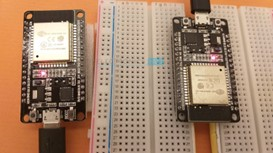
\includegraphics[width=10cm]{1.jpg}};
                \end{tikzpicture}
            \end{figure}


        Why the built-in Bluetooth Low Energy chip in ESP32? 
        \begin{itemize}
            \item \textbf{Low power consumption:} \\
            Bluetooth Low Energy is designed to be highly energy-efficient, allowing devices to operate on a small battery for long periods of time. This makes it the best suited communication protocol for low-power devices like the ESP32.

            \item \textbf{Short-range communication:}\\ 
            BLE is designed for short-range communication, which means that it is ideal for use in the “Metroband”.

            \item \textbf{Compatibility:} \\ 
            BLE is widely adopted and supported by most modern smartphones, making it easy to communicate with a wide range of devices.

            \item \textbf{Easy to use:} \\
            Can easily add wireless communication to the project without the need for additional hardware because of the built-in BLE chip.
        \end{itemize}

        Related problems and the solutions:
        \begin{itemize}
            \item \textbf{Interference:} \\
            BLE operates in the same frequency band as other wireless devices, which means that it may be subject to interference from other wireless signals. But the frequency ranges that are probable in concerts and bands do not belong to the range of the BLE frequency range. Also, Bluetooth is used in this device to send a unit pulse which will not be much affected by the other signals. For example:
            \begin{itemize}
                \item Wireless Microphones: 516-558 MHz
                \item In-Ear Monitors: 470-952 MHz
                \item Wireless Intercom Systems: 470-698 MHz
            \end{itemize}

            \item \textbf{Complexity:} 
            BLE can be more complex to implement than other wireless communication protocols but due to in built libraries in ESP 32 Bluetooth module can be accessed easily.
        \end{itemize}





        \subsection{Better battery - Polymer 3.7V 150mAh 401530 Lithium Ion Battery}

        \begin{figure}[!htb]
                \centering
                \begin{tikzpicture}
                    \node at (0.5,-0.2){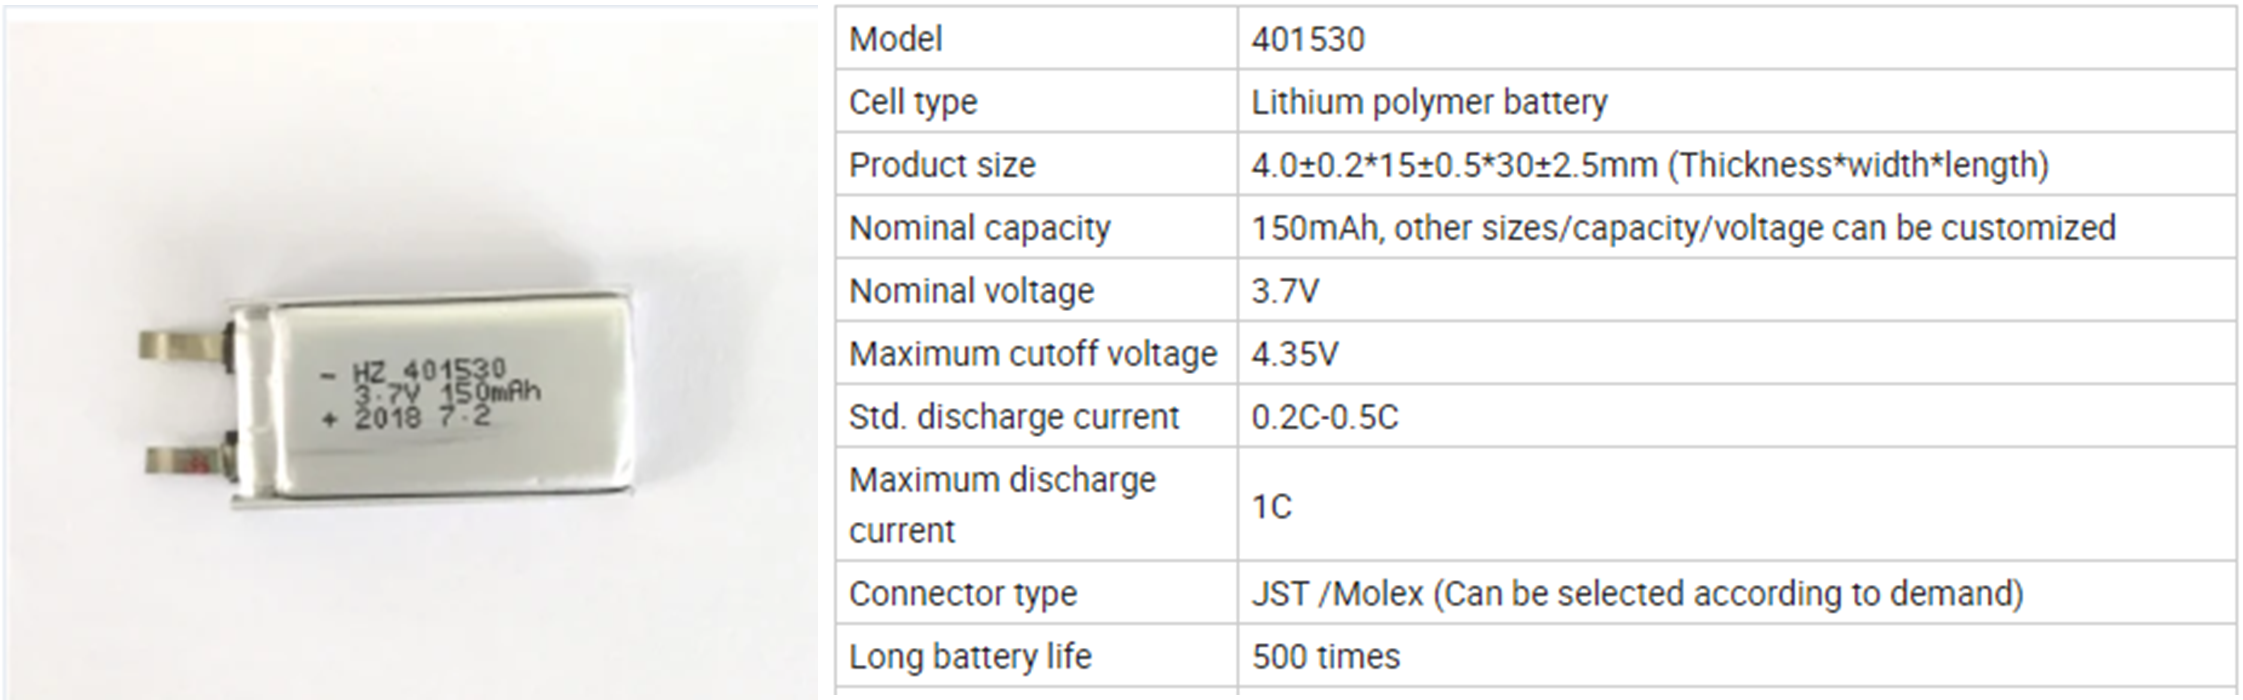
\includegraphics[width=15cm]{2.png}};
                \end{tikzpicture}
            \end{figure}

        Why Polymer 3.7V 150mAh 401530 Lithium Ion Battery?

        \begin{itemize}
            \item \textbf{High energy density:} \\
            Polymer batteries have a higher energy density than other types of batteries, meaning they can store more energy per unit of volume, allowing for longer battery life in a small form factor.

            \item \textbf{Low self-discharge rate:} \\
            Polymer batteries have a lower self-discharge rate than other types of batteries, meaning they can hold their charge for longer periods without losing significant energy.

            \item \textbf{Lightweight and compact:}\\ 
            Polymer batteries are very lightweight and can be molded into various shapes and sizes, making them an ideal choice for small wearable devices like smartwatches.
        \end{itemize}

        Related problems and the solutions:
        \begin{itemize}
            \item \textbf{Limited lifespan and Vulnerable to high temperatures:}\\
            One solution to prolong the lifespan of the polymer battery is to avoid exposing it to high temperatures, which can cause the battery to degrade faster.  \\
            Moreover, Heats pads and ventilating slots in the enclosure can be designed to overcome the above issues. Additionally, using the correct charging method and avoiding overcharging or discharging the battery can help extend its lifespan.

            \item \textbf{Risk of overcharging:}\\ 
            To avoid overcharging the battery a TP4056 - SOIC8 - Li-on Battery Charger IC 1A is used(https://www.sunrom.com/p/tp4056-li-on-battery-charger-ic-1a). It helps prevent overcharging by using a constant-current charging method, including built-in overcharging protection, and an auto-termination feature. This helps ensure that the battery is charged safely and optimally, without the risk of overcharging.

            \begin{figure}[!htb]
                \centering
                \begin{tikzpicture}
                    \node at (0.5,-0.2){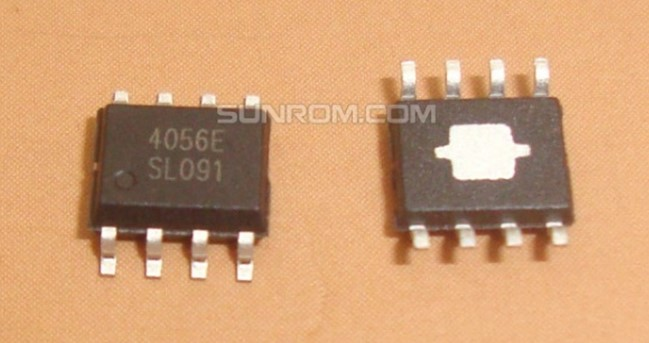
\includegraphics[width=10cm]{3.jpg}};
                \end{tikzpicture}
            \end{figure}
            
            \item \textbf{Output voltage from the IC is not enough to drive the motor:}\\
            Output from the GPIO pins of the module can give only 40 mA when the vibration motor requires 75 mA to run, which means to start it requires an even larger current. Since connecting the motor directly to module can damage the module as well as it might result in motor not starting up at certain orientation. As a solution for this we can give the output from the module to the base of a transistor and use it as a switch.
        \end{itemize}
  

        \section{Timing}
        Singular core micro controller processes sequentially, but in the Metroband as we need certain tasks to be done simultaneously, we are restricted from achieving this. Moreover, it affects the processing speed as a single-core microcontroller may not be able to process data leading to slower response times and potential inaccuracies in measuring the user's BPM. Furthermore, the functionality also becomes limited as a single-core microcontroller may not have the necessary resources to handle complex algorithms or multiple inputs and outputs. \\
        
        But there is a trade off in using multicores as the power consumption increases with the increasing number of cores. \\
        
        These issues can be overcome by:
        
        \subsection{Using a Dual core microcontroller - ESP-32S WiFi Bluetooth Dual Mode Module (MD0271)}

        \begin{figure}[htpb]
                \centering
                \begin{tikzpicture}
                    \node at (0.5,-0.2){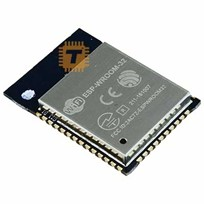
\includegraphics[width=4cm]{4.jpg}};
                \end{tikzpicture}
            \end{figure}

        Why ESP-32S WiFi Bluetooth Dual Mode Module (MD0271)

        \begin{itemize}
            \item \textbf{Improved performance:}\\ 
            With two cores, the microcontroller can handle multiple tasks simultaneously, improving the overall performance of the wristband.
            
            \item \textbf{More functionality:} \\
            This microcontroller can handle more complex algorithms, multiple inputs, and outputs, enabling the Metroband to perform more functions than a single-core microcontroller.

            \item \textbf{Enhanced responsiveness:} \\
            With multiple cores, the wristband can more quickly respond to user inputs or changes in BPM, improving overall user experience.
        \end{itemize}


        \section{Vibrations}
        The device gives the tempo with vibrations, and since all the components need to be packed into a small compartment, other components including the PCB would constantly be subjected to vibrations. And these vibrations cannot be made less intense as that would mean it would be harder for the user to sense the vibrations.\\
        
        These issues can overcome by using these strategies:
        
        \subsection{Using High Density Polyethylene/ polypropylene or Acrylonitrile Butadiene Styrene for the back plate.}
        
        Why High-Density Polyethylene/ polypropylene or Acrylonitrile Butadiene Styrene?

        \begin{itemize}
            \item \textbf{Feels vibrations more effectively:}\\
            User feels vibrations more effectively because of their unique properties.

            \item \textbf{Durability:} \\
            HDPE, PP, and ABS are all known for their toughness and durability. They are resistant to impact, abrasion, and chemicals, making them ideal for use in a wristband that may be exposed to rough conditions or frequent use.

            \item \textbf{Lightweight:} \\
            HDPE, PP, and ABS are all lightweight materials, which can help keep the overall weight of the wristband low and comfortable to wear.

            \item \textbf{Cost-effective:} \\
            These materials are relatively inexpensive compared to other materials such as metals or composites, which can help keep the overall cost of manufacturing the wristband low.
        \end{itemize}

        \subsection{Separate the vibrating motor and the PCB with butyl rubber:}

        \begin{itemize}
            \item \textbf{Vibration isolation:} \\
            Butyl rubber is a good vibration-damping material, which means that it can absorb and dampen the vibrations produced by the motor. By isolating the motor from the PCB with butyl rubber, the vibrations are less likely to affect the electronic components on the PCB, which can help improve the reliability and longevity of the wristband.

            \item \textbf{Shock absorption:} \\
            In addition to absorbing vibrations, butyl rubber can also absorb shocks and impacts, which can be important in a wristband that may be subjected to rough handling or impacts.
            
            \item \textbf{Noise reduction:} \\ 
            By absorbing and damping the vibrations produced by the motor, butyl rubber can also help reduce the amount of noise generated by the motor, which can improve the overall user experience.
        \end{itemize}

        \subsection{Vibration motor section can be fixed to the back plate and PCB and display unit to the front plate.} 
 
        The PCB is not allowed to be subjected to vibrations as it fastened to the front layer since the vibrating motor section is fixed to the back plate. At the joint of the back plate and the front layer vibrations can be damped out using rubber railing.


        \section{Overall size of the product}
        The overall size of the Metroband is an important factor to consider when designing it because it affects both the user experience and the technical aspects of the device. As it needs to be worn in hand, and signifies the tempo using vibrations, and as it needs to be easy to use and not interrupt the activity of playing an instrument the size of it becomes a constraint.\\
        
        To overcome the challenges associated with the size of the Metroband, we can use the following strategies:

        \begin{itemize}
            \item \textbf{Minimizing component size:}\\
            The size of the components used in the Metroband can be reduced as possible. Such as:
            \begin{compactitem}
                \item Smaller batteries (Polymer Battery 3.7V 150mAh 401530 Lithium Ion Battery)
                \item SMD components
                \item Coin vibrating motor 
            \end{compactitem}


            \item \textbf{Using compact designs:}\\
            The design can be compacted to make the most of the available space. This may involve using a square display to maximize screen space.

            \item \textbf{Prioritizing key features:}\\
            The key features that users are most likely to use can be prioritized and the design of the Metroband around those features is optimized. This may involve sacrificing some features or functionality to reduce the overall size of the device.
        \end{itemize}


\end{document}